\chapter{Arhitektura i dizajn sustava}
		
		\textbf{\textit{dio 1. revizije}}\\

		\textit{ Potrebno je opisati stil arhitekture te identificirati: podsustave, preslikavanje na radnu platformu, spremišta podataka, mrežne protokole, globalni upravljački tok i sklopovsko-programske zahtjeve. Po točkama razraditi i popratiti odgovarajućim skicama:}
	\begin{itemize}
		\item 	\textit{izbor arhitekture temeljem principa oblikovanja pokazanih na predavanjima (objasniti zašto ste baš odabrali takvu arhitekturu)}
		\item 	\textit{organizaciju sustava s najviše razine apstrakcije (npr. klijent-poslužitelj, baza podataka, datotečni sustav, grafičko sučelje)}
		\item 	\textit{organizaciju aplikacije (npr. slojevi frontend i backend, MVC arhitektura) }		
	\end{itemize}

	
		

		

				
		\section{Baza podataka}
		U aplikaciji će baza podataka bit prikazana relacijskim modelom podataka. Objekti relacijskog modela su relacije, a svaka ima jedinstveno ime unutar sheme baze podataka. Relacija je tablica čiji se imenovani stupci nazivaju atributi, a redci n-torke. Ključ entiteta je skup atributa koji jednoznačno određuje entitet. U našem sustavu entiteti baze podataka su:
	\begin{itemize}
		\item Rad
		\item Autor
		\item Konferencija
		\item Korisnik
		\item Prisutan\_na
		\item Mjesto
		\item Fotografija
		\item Admin
		\item Pokrovitelj	
		\item Pokrovitelj\_na	
	\end{itemize}
			\subsection{Opis tablica}
			Entitet \textbf {Rad} sadrži sve važne informacije o radu. Sadrži atribute: ID rada, naziv postera, naziv prezentacije, naslov rada, OIB autora, ID konferencije na koju je prijavljen i ukupan broj osvojenih glasova na toj konferenciji. Atribut naziv prezentacije je opcionalan te stoga može poprimiti vrijednost null. Entitet Rad u binarnoj je vezi s \textit{(Many-to-One)} s entitetom Konferencija i u vezi \textit{(Many-to-One)} s entitetom Autor.
				\begin{longtblr}[
					label=none,
					entry=none
					]{
						width = \textwidth,
						colspec={|X[6,l]|X[6, l]|X[20, l]|}, 
						rowhead = 1,
					} %definicija širine tablice, širine stupaca, poravnanje i broja redaka naslova tablice
					\hline \SetCell[c=3]{c}{\textbf{Rad}}	 \\ \hline[3pt]
					\SetCell{LightGreen}idRad & SERIAL	&  	jedinstveni identifikator rada 	\\ \hline
					nazivPoster	& VARCHAR &   	naziv postera koji prikazuje rad\\ \hline 
					nazivPptx & VARCHAR &   naziv prezentacije koja prikazuje rad, može biti null\\ \hline 
					naslov & VARCHAR	&    naslov rada\\ \hline 
					ukupnoGlasova & INT &   ukupan broj osvojenih glasova na konferenciji\\ \hline 
					\SetCell{LightBlue}idKonf	& SERIAL &   	jedinstveni identifikator konferencije\\ \hline 
					\SetCell{LightBlue}OIB & INT	&    osobni identifikacijski broj autora\\ \hline 
				\end{longtblr}						
			
			\noindent Entitet \textbf {Autor} sadrži informacije o autoru. Sadrži atribute: OIB autora, email autora i ime i prezime autora. Entitet Autor u binarnoj je vezi s entitetom Rad \textit{(One-to-Many)}.
				\begin{longtblr}[
					label=none,
					entry=none
					]{
						width = \textwidth,
						colspec={|X[6,l]|X[6, l]|X[20, l]|}, 
						rowhead = 1,
					} %definicija širine tablice, širine stupaca, poravnanje i broja redaka naslova tablice
					\hline \SetCell[c=3]{c}{\textbf{Autor}}	 \\ \hline[3pt]
					\SetCell{LightGreen}OIB & INT	&  	osobni identifikacijski broj autora \\ \hline
					emailAutor	& VARCHAR &   	email autora\\ \hline 
					ime & VARCHAR &   ime autora\\ \hline 
					prezime & VARCHAR	&    prezime autora\\ \hline 
				\end{longtblr}		

			\noindent Entitet \textbf {Konferencija} sadrži informacije o stručnoj konferenciji koja će se održati. Sadrži atribute: ID konferencije, poveznica na video prijenos konferencije, pin za ulazak na konferenciju, vrijeme početka i vrijeme kraja konferencije, ID admina zaduženog za konferenciju i poštanski broj mjesta u kojem se održava konferencija. Entitet Konferencija u binarnoj je vezi s entitetom Rad \textit{(One-to-Many)}, u binarnoj vezi \textit{(Many-to-Many)} s entitetom Korisnik, u vezi \textit{(Many-to-One)} s entitetom Mjesto, \textit{(One-to-Many)} s entitetom Fotografija, \textit{(Many-to-One)} s entitetom Admin i \textit{(Many-to-Many)} s entitetom Pokrovitelj.
				\begin{longtblr}[
					label=none,
					entry=none
					]{
						width = \textwidth,
						colspec={|X[6,l]|X[6, l]|X[20, l]|}, 
						rowhead = 1,
					} %definicija širine tablice, širine stupaca, poravnanje i broja redaka naslova tablice
					\hline \SetCell[c=3]{c}{\textbf{Konferencija}}	 \\ \hline[3pt]
					\SetCell{LightGreen}idKonf & SERIAL	&  	jedinstveni identifikator konferencije \\ \hline
					urlVideo	& VARCHAR &   	 poveznica na direktno video praćenje
trenutnih događanja u glavnoj konferencijskoj dvorani\\ \hline 
					pin & INT &   jedinstveni pin konferencije\\ \hline 
					vrijemePocetak & TIMESTAMP	&    početak konferencije\\ \hline 
					vrijemeKraj & TIMESTAMP	&    kraj konferencije\\ \hline 
					\SetCell{LightBlue} idAdmin & SERIAL &   jedinstveni identifikator admina zaduženog za konferenciju\\ \hline 
					\SetCell{LightBlue} pbr & INT &   poštanski broj mjesta u kojem se održava konferencija\\ \hline 
				\end{longtblr}		

			\noindent Entitet \textbf {Korisnik} sadrži informacije o korisniku aplikacije. Sadrži atribute: ID korisnika, email korisnika i lozinka korisnika. Entitet Korisnik u binarnoj je vezi s entitetom Konferencija \textit{(Many-to-Many)}.
				\begin{longtblr}[
					label=none,
					entry=none
					]{
						width = \textwidth,
						colspec={|X[7,l]|X[6, l]|X[20, l]|}, 
						rowhead = 1,
					} %definicija širine tablice, širine stupaca, poravnanje i broja redaka naslova tablice
					\hline \SetCell[c=3]{c}{\textbf{Korisnik}}	 \\ \hline[3pt]
					\SetCell{LightGreen}idKorisnik & SERIAL	&  	jedinstveni identifikator korisnika \\ \hline
					emailKorisnik 	& VARCHAR &   	email korisnika\\ \hline 
					lozinkaKorisnik & VARCHAR &   hash lozinke korisnika\\ \hline 
				\end{longtblr}	

			\noindent Entitet \textbf {Prisutan\_na} sadrži informacije o prisutnosti pojedinog korisnika na određenoj konferenciji te je li glasao na njoj ili ne. Sadrži atribute: ID konferencije, ID korisnika i glasao. Entitet Prisutan\_na rezultat je binarne veze \textit{(Many-to-Many)} entiteta Korisnik i Konferencija.
				\begin{longtblr}[
					label=none,
					entry=none
					]{
						width = \textwidth,
						colspec={|X[6,l]|X[6, l]|X[20, l]|}, 
						rowhead = 1,
					} %definicija širine tablice, širine stupaca, poravnanje i broja redaka naslova tablice
					\hline \SetCell[c=3]{c}{\textbf{Prisutan\_na}}	 \\ \hline[3pt]
					\SetCell{LightGreen}idKonf & SERIAL	&  	jedinstveni identifikator konferencije \\ \hline
					\SetCell{LightGreen}idKorisnik	& SERIAL &   	jedinstveni identifikator korisnika\\ \hline 
					glasao & BOOLEAN &   informacija je li korisnik već glasao na konferenciji\\ \hline 
				\end{longtblr}

			\noindent Entitet \textbf {Mjesto} sadrži informacije o pojedinom mjestu. Sadrži atribute: poštanski broj i naziv mjesta. Entitet Mjesto u binarnoj je vezi s entitetom Konferencija \textit{(One-to-Many)}. 
				\begin{longtblr}[
					label=none,
					entry=none
					]{
						width = \textwidth,
						colspec={|X[6,l]|X[6, l]|X[20, l]|}, 
						rowhead = 1,
					} %definicija širine tablice, širine stupaca, poravnanje i broja redaka naslova tablice
					\hline \SetCell[c=3]{c}{\textbf{Mjesto}}	 \\ \hline[3pt]
					\SetCell{LightGreen}pbr & INT &   poštanski broj mjesta \\ \hline
					naziv	& VARCHAR &   	naziv mjesta\\ \hline 
				\end{longtblr}

			\noindent Entitet \textbf {Fotografija} sadrži informacije o uslikanoj fotografiji te na kojoj konferenciji je uslikana. Sadrži atribute: ID fotografije, naziv fotografije i ID konferencije. Entitet Fotografija u binarnoj je vezi s entitetom Konferencija \textit{(Many-to-One)}. 
				\begin{longtblr}[
					label=none,
					entry=none
					]{
						width = \textwidth,
						colspec={|X[6,l]|X[6, l]|X[20, l]|}, 
						rowhead = 1,
					} %definicija širine tablice, širine stupaca, poravnanje i broja redaka naslova tablice
					\hline \SetCell[c=3]{c}{\textbf{Fotografija}}	 \\ \hline[3pt]
					\SetCell{LightGreen}idFoto & SERIAL	&  	jedinstveni identifikator fotografije\\ \hline
					naziv	& VARCHAR &   	naziv fotografije\\ \hline 
					\SetCell{LightBlue}idKonf & SERIAL &   jedinstveni identifikator konferencije\\ \hline 
				\end{longtblr}

			\noindent Entitet \textbf {Admin} sadrži informacije adminima. Sadrži atribute: ID admina, email i lozinka admina. Entitet Admin u binarnoj je vezi s entitetom Konferencija \textit{(One-to-Many)}. 
				\begin{longtblr}[
					label=none,
					entry=none
					]{
						width = \textwidth,
						colspec={|X[6,l]|X[6, l]|X[20, l]|}, 
						rowhead = 1,
					} %definicija širine tablice, širine stupaca, poravnanje i broja redaka naslova tablice
					\hline \SetCell[c=3]{c}{\textbf{Admin}}	 \\ \hline[3pt]
					\SetCell{LightGreen}idAdmin & SERIAL	&  	jedinstveni identifikator admina\\ \hline
					emailAdmin	& VARCHAR &   	email admina\\ \hline 
					lozinkaAdmin & VARCHAR &   hash lozinke admina\\ \hline 
				\end{longtblr}

			\noindent Entitet \textbf {Pokrovitelj} sadrži informacije o pokrovitelju. Sadrži atribute: ID pokrovitelja,  url stranice pokrovitelja i naziv pokrovitelja. Entitet Pokrovitelj u binarnoj je vezi s entitetom Konferencija \textit{(Many-to-Many)}. 
				\begin{longtblr}[
					label=none,
					entry=none
					]{
						width = \textwidth,
						colspec={|X[7,l]|X[6, l]|X[20, l]|}, 
						rowhead = 1,
					} %definicija širine tablice, širine stupaca, poravnanje i broja redaka naslova tablice
					\hline \SetCell[c=3]{c}{\textbf{Pokrovitelj}}	 \\ \hline[3pt]
					\SetCell{LightGreen}idPokrovitelj & SERIAL	&  	jedinstveni identifikator pokrovitelja\\ \hline
					urlPokrovitelj	& VARCHAR &   	poveznica na stranicu pokrovitelja\\ \hline 
					nazivPokrovitelj	& VARCHAR &   	naziv pokrovitelja\\ \hline 
				\end{longtblr}

			\noindent Entitet \textbf {Pokrovitelj\_na} sadrži informacije o uključenosti pokrovitelja na pojedinoj konferenciji. Sadrži atribute: ID konferencije i ID pokrovitelja. Entitet Pokrovitelj\_na rezultat je binarne veze \textit{(Many-to-Many)} entiteta Pokrovitelj i Konferencija.
				\begin{longtblr}[
					label=none,
					entry=none
					]{
						width = \textwidth,
						colspec={|X[6,l]|X[6, l]|X[20, l]|}, 
						rowhead = 1,
					} %definicija širine tablice, širine stupaca, poravnanje i broja redaka naslova tablice
					\hline \SetCell[c=3]{c}{\textbf{Pokrovitelj\_na}}	 \\ \hline[3pt]
					\SetCell{LightGreen}idKonf & SERIAL	&  	jedinstveni identifikator konferencije \\ \hline
					\SetCell{LightGreen}idPokrovitelj	& SERIAL &   	jedinstveni identifikator pokrovitelja\\ \hline 
				\end{longtblr}
	
			\subsection{Dijagram baze podataka}
				\textit{ U ovom potpoglavlju potrebno je umetnuti dijagram baze podataka. Primarni i strani ključevi moraju biti označeni, a tablice povezane. Bazu podataka je potrebno normalizirati. Podsjetite se kolegija "Baze podataka".}
					\begin{figure}[H]
						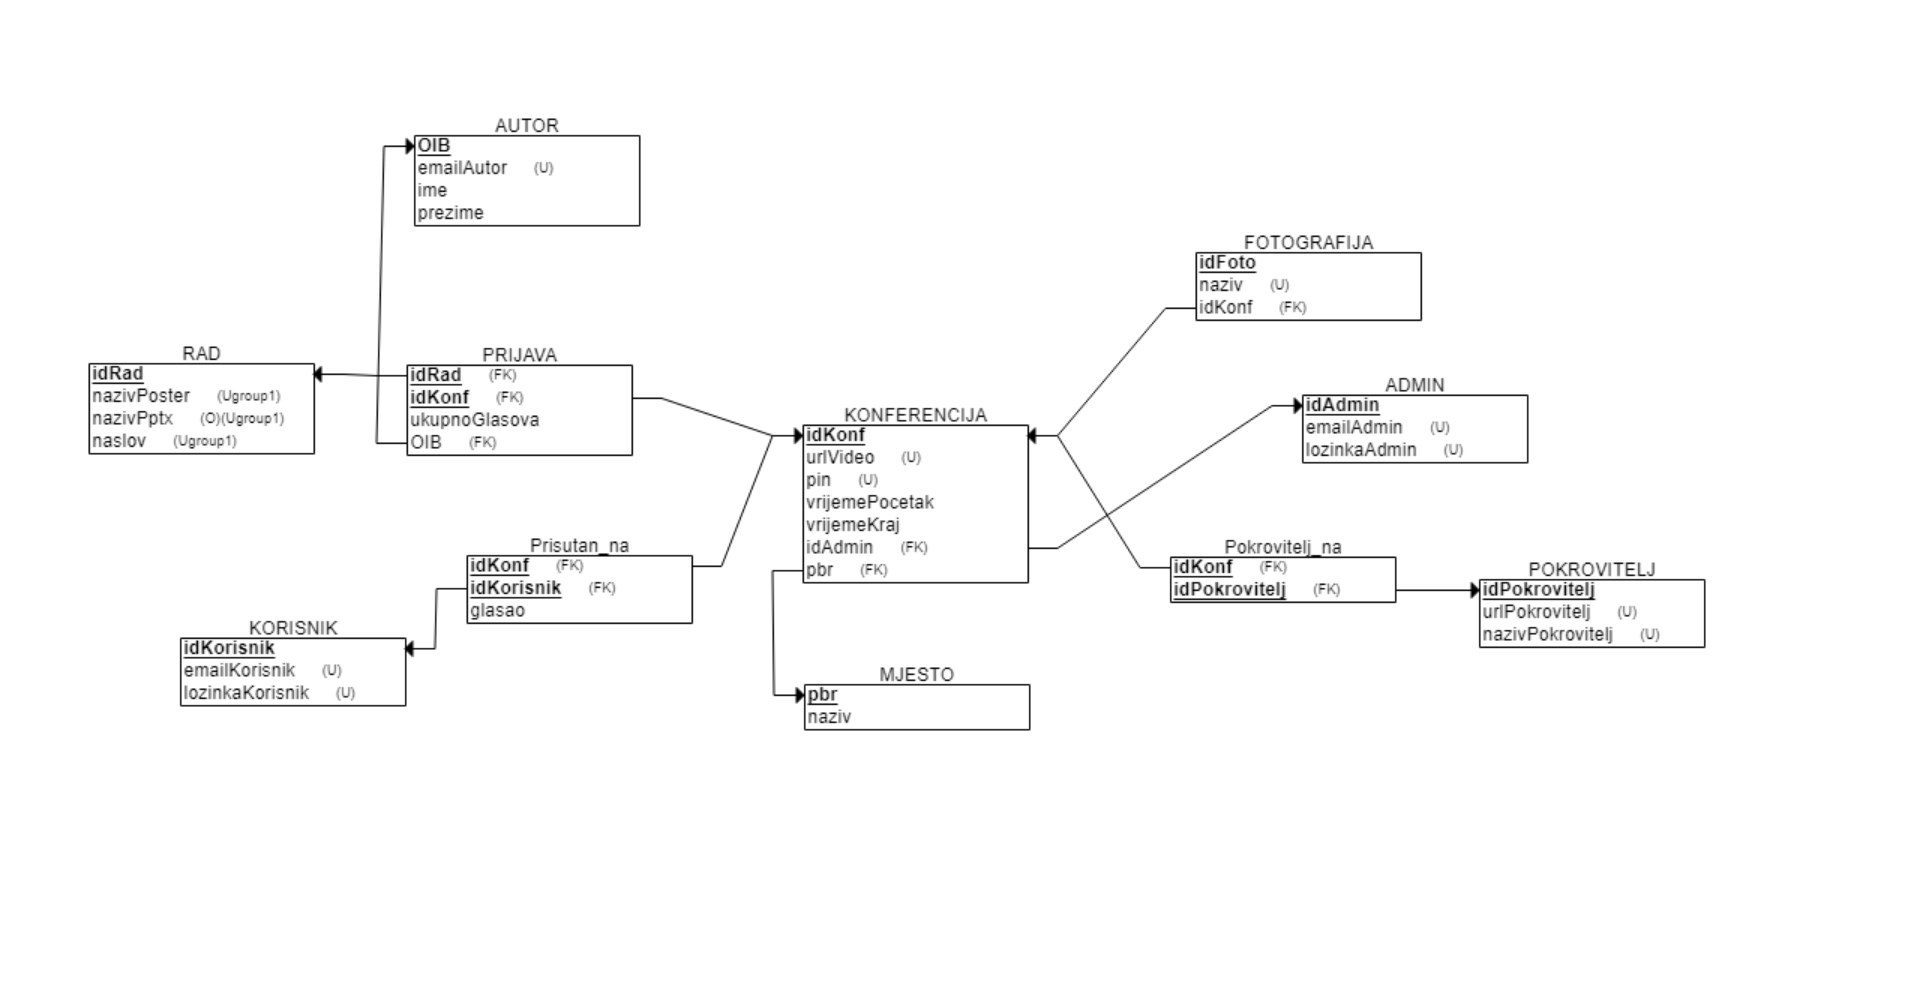
\includegraphics[scale=0.55]{slike/dijagram baze podataka.PNG} %veličina slike u odnosu na originalnu datoteku i pozicija slike
						\centering
						\caption{Dijagram baze podataka}
						\label{fig:promjene3}
					\end{figure}			
			\eject
			
			
		\section{Dijagram razreda}
		
			\textit{Potrebno je priložiti dijagram razreda s pripadajućim opisom. Zbog preglednosti je moguće dijagram razlomiti na više njih, ali moraju biti grupirani prema sličnim razinama apstrakcije i srodnim funkcionalnostima.}\\
			
			\textbf{\textit{dio 1. revizije}}\\
			
			\textit{Prilikom prve predaje projekta, potrebno je priložiti potpuno razrađen dijagram razreda vezan uz \textbf{generičku funkcionalnost} sustava. Ostale funkcionalnosti trebaju biti idejno razrađene u dijagramu sa sljedećim komponentama: nazivi razreda, nazivi metoda i vrste pristupa metodama (npr. javni, zaštićeni), nazivi atributa razreda, veze i odnosi između razreda.}\\
			
			\textbf{\textit{dio 2. revizije}}\\			
			
			\textit{Prilikom druge predaje projekta dijagram razreda i opisi moraju odgovarati stvarnom stanju implementacije}
			
			
			
			\eject
		
		\section{Dijagram stanja}
			
			
			\textbf{\textit{dio 2. revizije}}\\
			
			\textit{Potrebno je priložiti dijagram stanja i opisati ga. Dovoljan je jedan dijagram stanja koji prikazuje \textbf{značajan dio funkcionalnosti} sustava. Na primjer, stanja korisničkog sučelja i tijek korištenja neke ključne funkcionalnosti jesu značajan dio sustava, a registracija i prijava nisu. }
			
			
			\eject 
		
		\section{Dijagram aktivnosti}
			
			\textbf{\textit{dio 2. revizije}}\\
			
			 \textit{Potrebno je priložiti dijagram aktivnosti s pripadajućim opisom. Dijagram aktivnosti treba prikazivati značajan dio sustava.}
			
			\eject
		\section{Dijagram komponenti}
		
			\textbf{\textit{dio 2. revizije}}\\
		
			 \textit{Potrebno je priložiti dijagram komponenti s pripadajućim opisom. Dijagram komponenti treba prikazivati strukturu cijele aplikacije.}